\section{Solution, our Approach to RRP(G, v, R)}

{The solution is two fold, first we preprocess the data and create an index. Then we use a modified A* algorithm to traverse the graph using the index and answer any query.}

{We will use a running example to explain the main idea and then formally present an algorithm. Consider Figure \ref{fig:space-partitioned} which has a social graph of friends and their check ins at various restaurants.}

\begin{figure}[t]
	\centering 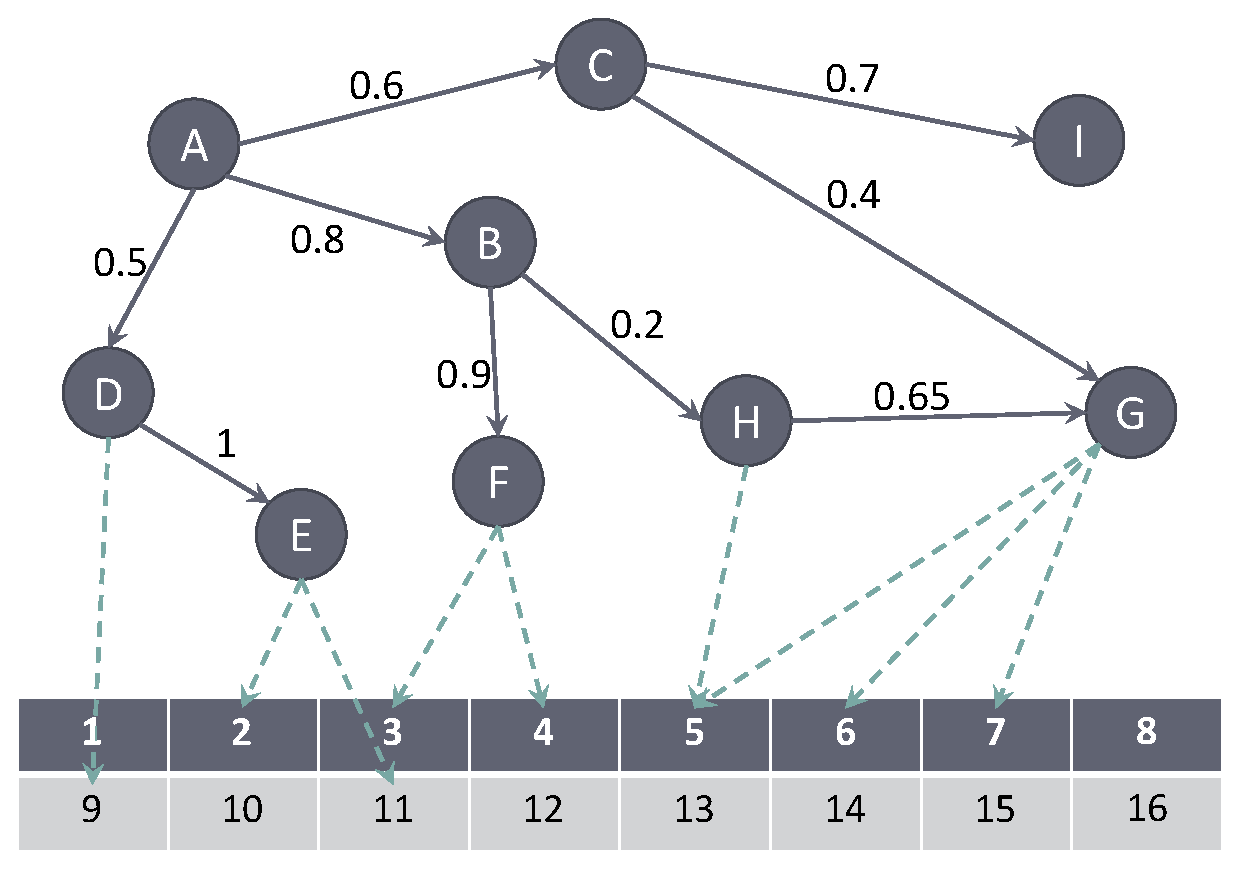
\includegraphics[width=0.40\textwidth]{images/space_partitioned_world.eps}
    \caption{Space partitioned world}
    \label{fig:space-partitioned}
\end{figure}

{In Figure \ref{fig:space-partitioned}, each vertex symbolizes a person and two nodes are connected if there is a social relationship between them. The number on the edge indicates their social distance, lesser implies stronger bond. Forest green edges from the nodes to the map are all check-ins made by people at various restaurants, which are our spatial vertices. }

\subsection{Building the index, GeoReachPaths}

\subsubsection{Structure}
The goal of the index is to quickly prune the graph for any range predicate and a source vertex. Therefore for every vertex we add some spatial and social meta information. Using this meta information, the traversal algorithm at query time can decide whether to visit a sub-graph starting at that node or not.

Using the spatial attributes of the vertices, we create the spatial meta information. We divide the world into a fixed number of blocks in space and number the blocks. Then for each restaurant (i.e. spatial node) we update the meta information for all the people nodes (other vertices) who have checked-in there with the block number where the restaurant belongs. If the world is divided into very fine blocks, each meta entry can be really huge. To compress the index entry, we divide the world again but this time into more coarser blocks and number them. For all the index entries which cross a threshold, we update its block numbers to this coarser division. We repeat this recursively until the threshold is satisfied. Once we have this in place, at query time, while traversing the graph for finding a shortest path, we can straight away prune away traversing sub-graphs starting at a vertex which does not reach the region of interest.

Using the social distances (edge weights) we create social meta information/index. We pick a few vertices from our graph based on some criteria (detailed later) and store shortest distance from each to all vertices it can reach using well known single source shortest algorithms like Dijkstra's. Lets call these selected vertices as landmarks. So social meta information is a table which has shortest distances information from each landmark. Using these landmarks and traingle inequality we obtain an estimate of the shortest distance from any vertex to any other vertex in the graph. This valuable information is used during graph traversal to prune sub-graphs even better and will be details in section \ref{querying}.

\subsubsection{Using the Spatial Component}
In to our running example, we divide the entire region into equal sized blocks from 1 to 16 as show in Figure \ref{fig:space-partitioned}. Then for vertex D, meta information would be {[}8{]} as the user checked-in at a restaurant which falls in block number 8. Similarly for vertex G, the meta information would be {[}5, 6, 7{]}. Continuing like this, we populate a meta information table for each vertex which are directly connected to a spatial node.

% \begin{table}[h]
% 	\caption{1-hop reachability meta table}
% 	\label{tab:1-hop-meta}
% 	\begin{center}
% 		\renewcommand{\arraystretch}{1.25}
% 		\begin{tabular}{ c | c }
% 			\hline
% 			Vertex & Reachable Block Numbers \\ \hline
% 			\hline
% 			D & [8] \\
% 			E & [2, 10] \\
% 			F & [3, 4] \\
% 			H & [5] \\
% 			G & [5, 6, 7] \\
% 			\hline
% 		\end{tabular}
% 	\end{center}
% \end{table}

This is the reachability to restaurants by 1-hop which can answer 1-hop queries. For example, did vertex G check-in at restaurant L1 or did vertex E visit any restaurant in a region L2. The first can be answered by using location of L1, we can find the block number and cross-reference if that block number is listed under G in the meta table. We will see more details in the next section where we talk about answering queries.

If we extend the idea of 1-hop reachability to any number of hops, it is multi-hop reachability or simply reachability. These values denote all blocks that are reachable from a vertex in any number of hops/steps. For building multi-hop reachability information, we reverse the direction of all the edges. Now, for every vertex, we append it reachability information to all the vertices it is directly connected to bottom up.

Assume we inverse the graph by reversing direction of all edges in it. Now to compute multi-hop meta information for H, we append G's meta information. Similarly for B, we append meta information from H and F. As this is a DAG, we have complete reachability information of every node after completing the exercise for entire graph. The final meta table for every node looks like the one shown in the column 1 of Table \ref{tab:multi-hop-meta}.

\begin{table}[h]
	\caption{Meta table for multi-hop reachability}
	\label{tab:multi-hop-meta}
	\begin{center}
		\renewcommand{\arraystretch}{1.25}
		\begin{tabular}{ c | c | c }
			\hline
			Vertex & Reachable Block Numbers & Compressed\\ \hline
			\hline
			D & [9, 2, 11] & [17, 18] \\
			E & [2, 11] & [2, 11] \\
			F & [3, 4] & [3, 4] \\
			H & [5, 6, 7] & [19, 20] \\
			G & [5, 6, 7] & [19, 20] \\
			C & [5, 6, 7] & [19, 20] \\
			B & [3, 4, 5, 6, 7] & [18, 19, 20] \\
			A & [3, 4, 5, 6, 7] & [18, 19, 20] \\
			\hline
		\end{tabular}
	\end{center}
\end{table}

Using this table we can answer any region reachability query which will be described in the next section. Now we can see that vertex A can reach whatever B, C and D can reach. Similarly B can reach whatever H and F can reach and so on. However, as you can see the size of the meta table (a.k.a index table) can grow really large as vertices like B and A which are highly connected can reach many blocks.

In order to compress the entries in our meta table for highly reachable nodes, we add a new layer of blocks with higher resolution.

% \begin{figure}[h]
%     \centering
%     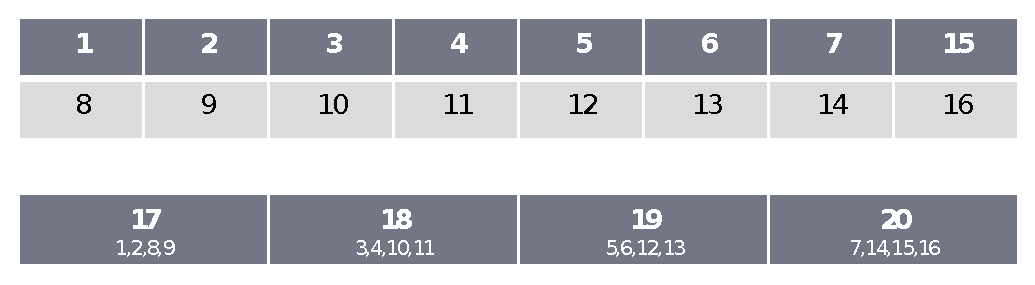
\includegraphics[width=0.8\linewidth]{images/image07.eps}
%     \caption{Multi layer grid index}
%     \label{fig:multi-grid}
% \end{figure}

{As shown in Figure \ref{fig:multi-grid2} (assume the 3rd layer does not exist for now), blocks 17 to 20 are added on top of blocks 1 to 16. Imagine this like a stack where the old layer sits exactly on top of the new layer. That is block 17 covers exactly the same area as area covered by blocks 1, 2, 8 and 9. Similarly block 18 in layer 1 represents blocks 3, 4, 10 and 11 of layer 0. Due to this change, our meta table becomes like the shown in the 3rd column of the Table \ref{tab:multi-hop-meta}

% \begin{table}[h]
% 	\caption{Compressed Meta table for multi-hop reachability}
% 	\label{tab:multi-hop-meta-compressed}
% 	\begin{center}
% 		\renewcommand{\arraystretch}{1.25}
% 		\begin{tabular}{ c | c }
% 			\hline
% 			Vertex & Reachable Block Numbers \\ \hline
% 			\hline
% 			D & [8] \\
% 			E & [2, 10] \\
% 			F & [3, 4] \\
% 			H & [\textbf{19, 20}] \\
% 			G & [\textbf{19, 20}] \\
% 			\textbf{C} & [\textbf{19, 20}] \\
% 			\textbf{B} & [\textbf{18, 19, 20}] \\
% 			\textbf{A} & [\textbf{18, 19, 20}] \\
% 			\hline
% 		\end{tabular}
% 	\end{center}
% \end{table}

To compress further we can add one more layer below layer 1 as show in Figure \ref{fig:multi-grid2}.

\begin{figure}[t]
    \centering
    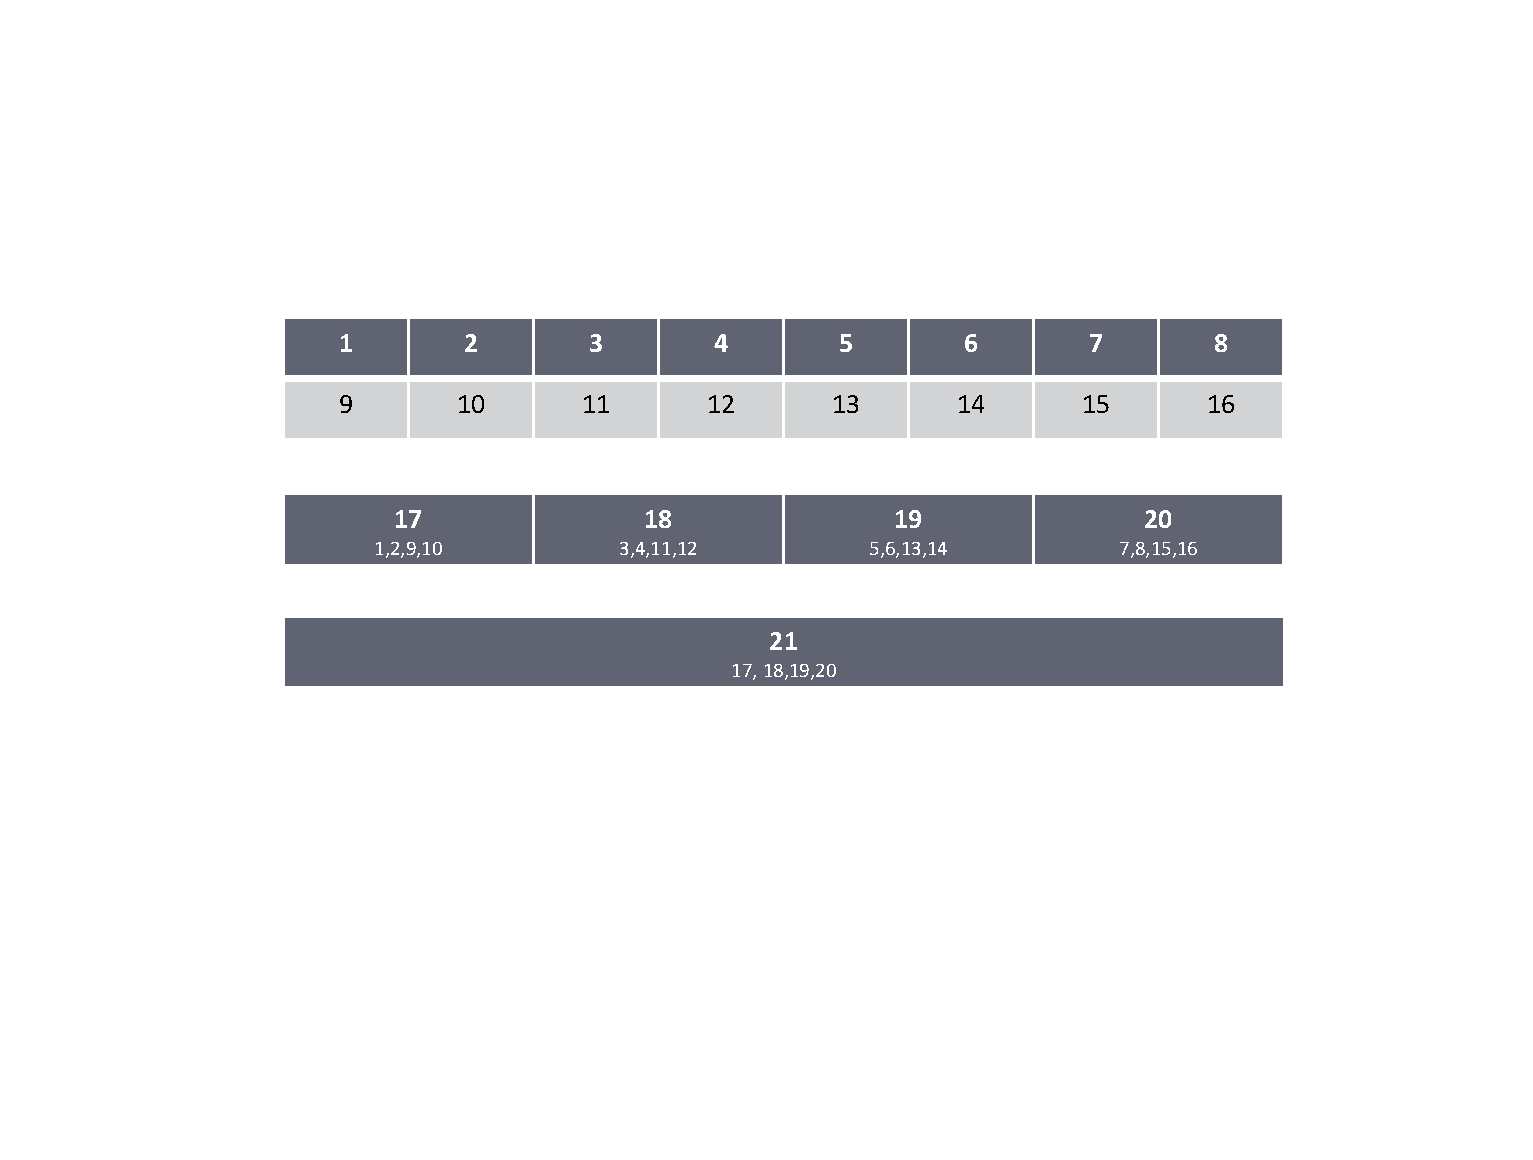
\includegraphics[width=0.88\linewidth]{images/multi_layer_grid_index.eps}
    \caption{Multi layer grid index}
    \label{fig:multi-grid2}
\end{figure}

Here block 21 represents blocks 17, 18, 19 and 20 in the layer above it. As you can see the reduction factor for every layer is set to one fourth which is a tunable parameter RF. The number of layers in the multi layer grid index is guided by another tunable parameter M. M is the maximum size, in terms of number of block ids, of meta information for a vertex. For example, if M = 2, then each vertex can only have two entries in its meta information and until we satisfy this limit, we create new layers.

% \begin{center}
% $Index Size \propto M \div RF$
% \end{center}
% \vspace{2mm}

\begin{lemma}
\label{vertex-component-meta}
{~Let v be a vertex in a connected component C of a graph G(V, E). Then,}

{\{$\forall v \in C$: Meta information of v = Meta information of C\}}\newline
\end{lemma}

\begin{proof}
In a connected component $C$, we can reach any vertex from any vertex by definition, i.e. $u \leadsto v, \forall (u, v) \in C$. 

If $C$ in condensed graph $G'$ can reach a set of regions $R$, then any vertex of $C$ can reach $R$ by definition of connected component.

Therefore, meta information of $C =$ meta information of $\forall v \in C$
\end{proof}

{We started the discussion by condensing G to a DAG (G'). Now we for
each node in a connected component we use the meta information of the
component from Lemma \ref{vertex-component-meta}.}

Then we will also construct a R-Tree using the spatial nodes in the graph. This will later be used at query time to filter the exact nodes in a region which will be discussed in the next section. These are the two indices created on the spatial component of the graph.

{Algorithm \ref{alg1} shows how the index, GeoReachPaths-spatial is created. In the first phase we add all spatial vertices as the meta information of the vertices they are connected from. Then we start a modified DFS to construct multi hop reachability. The REGION() method returns the block number for any spatial vertex. The REPARTITION() method ensures the }{M}{~constraint by recursively increasing the resolution by a factor of }{RF}{. In the DFS() method we recursively append meta information to the head vertex from the tail vertex.}

% \begin{algorithm*}[h]
% \caption{GeoReachPaths - spatial}
% \label{alg1}
% \begin{multicols}{2}
% \begin{algorithmic}[1]
% \State $MIN\_LAT \gets -90$
% \State $MAX\_LAT \gets 90$
% \State $MIN\_LNG \gets -180$
% \State $MAX\_LNG \gets 180$
% \State $DEFAULT\_RES \gets 10$ \Comment{Can be any positive integer}
% \State $AVAILABLE\_RES \gets [DEFAULT\_RES]$
% \State
% \Function{GeoReachPaths-Spatial}{$G, RF, M$}
%   \State $G' \gets DAG(G)$
%   \For{$v \gets G'.v:$}
%   	\State $v.meta \gets Set([])$   	\Comment{Initialize an empty set}
%   \EndFor
%   \State
%   \For{$u \gets spatial(G'.Adj(v))$}	 \Comment{1\-hop spatial reachability}
%   	\State v.meta.add(\Call{REGION}{u})
% 	\State \Call{REPARTITION}{v, RF, M}
%   \EndFor
%   \State
%   \State DO\_DFS(G', RF, M)  \Comment{multi\-hop region reachability}
% \EndFunction
% \State
% \Function{REGION}{$u$}
% 	\State $r \gets GET\_RES(u)$
% 	\State $cols \gets (MAX\_LAT - MIN\_LAT) \div r$
% 	\State \Return $floor(u.x \div r) + floor(u.y \div r)$
% \EndFunction
% \State
% \Function{REPARTITION}{$v, RF, M$}
% 	\If{$v.meta.size() \leq M$}
% 		\State \Return
% 	\EndIf
% 	\State $res \gets GET\_RES(v.meta[0])$
% 	\For{$r \gets v.meta$}
% 		\State \Call{TRANSLATE\_TO\_RES}{v.meta, $res \div MF$}
% 		\State \Call{REPARTITION}{v, RF, M}
% 	\EndFor
% \EndFunction
% \State
% \Function{DO\_DFS}{G, RF, M}
% 	\For{$v \gets G,V$}
% 		\State $v.visited \gets false$
% 	\EndFor
% 	\State
% 	\For{$v \gets G.V$}
% 		\State v.meta.add(\Call{DFS\_VISIT}{G, v})
% 		\State \Call{REPARTITION}{v, RF, M}
% 	\EndFor
% \EndFunction
% \State
% \Function{DFS\_VISIT}{G, v}
% 	\For{$u \gets G.Adj(v)$}
% 		\If{$v.visited = false$}
% 			\State v.meta.add(\Call{DFS\_VISIT}{G, u})
% 		\Else
% 			\State v.meta.add(u.meta)
% 		\EndIf
% 		\State \Call{REPARTITION}{v, RF, M}
% 		\State $v.visited \gets true$
% 		\State \Return v.meta
% 	\EndFor
% \EndFunction
% \end{algorithmic}
% \end{multicols}
% \end{algorithm*}

\begin{algorithm}[t]
\caption{GeoReachPaths - spatial}
\begin{scriptsize}
\label{alg1}
\begin{algorithmic}[1]
\Function{GeoReachPaths-Spatial}{$G, RF, M$}
  \State G' $\gets$ G.condense() \label{alg:condense}
  \For{v $\gets$ G.V} \Comment{1\-hop spatial reachability} \label{alg:onehopstart}
	  \For{u $\gets$ spatial(G'.Adj(v))}	 
	  	\State v.meta.add(\Call{REGION}{u})
	  \EndFor
	  \State \Call{REPARTITION}{v, RF, M}
  \EndFor \label{alg:onehopend}
  \State DO\_DFS(G', RF, M)  \Comment{multi\-hop region reachability} \label{alg:dfs}
\EndFunction
\Function{REGION}{$u$}
	\State \Return block \# for CURRENT\_RES(u)
\EndFunction
\Function{REPARTITION}{$v, RF, M$}
	\While{$v.meta.size() \leq M$}
		\State \Call{TRANSLATE\_TO\_RES}{v.meta, CURRENT\_RES(v) $\div$ RF}
	\EndWhile
\EndFunction
\Function{DO\_DFS}{G, RF, M}
	\For{$v \gets G.V$}
		\State v.meta.add(\Call{DFS\_VISIT}{G, v})
		\State \Call{REPARTITION}{v, RF, M}
	\EndFor
\EndFunction
\Function{DFS\_VISIT}{G, v}
	\For{$u \gets G.Adj($v) not $visited$}
		\State v.meta.add(\Call{DFS\_VISIT}{G, u})
	\EndFor
	\State \Return v.meta
\EndFunction
\end{algorithmic}
\end{scriptsize}
\end{algorithm}

\subsubsection{Using the social component}
Now we will use the social distances between nodes and create an index to prune the graph even better. This will take care of the cases when graph is very dense and the spatial index created before may not be of much use for pruning at query time. We will see more details in the next section on querying the graph.

The main idea is to select a few nodes in the graph and call them landmarks. Then for each vertex we compute shortest distances to each landmark and save them. Then at query time we will use these precomputed distances and triangle inequality to guide as a heuristic in the A* search algorithm. The inspiration is from \cite{AC2005} which introduces a class of algorithms called ALT. The main challenge here however is to find topK paths to a region unlike finding the shortest path from a given source to a given destination which is the main intent of the paper.

The quality of the landmarks determine the pruning power of the index. Choosing the right landmarks requires some domain knowledge of the graph. Once that is picked the process remains the same no matter what the graph represents. \cite{AC2005} talks about multiple ideas on how to find high quality landmarks quickly. The ideal case would be to find as minimum number of landmarks as possible such that every vertex in the graph is connected to at least one of the landmarks.  However leaving out a few vertices that do not reach any landmark will not hamper the correctness of the algorithm. Therefore finding the sweet spot of number of landmarks which gives the best query performance is crucial and is the main goal of \cite{AC2005}. The main contribution from our side is to use this social index and propose a new heuristic for A* algorithm.

Algorithm \ref{alg2}, GeoReachPaths-Social, describes how to create an index using landmarks. Landmark selection function on line 2 can be any of the functions described in \cite{AC2005}. Then for each landmark we compute the shortest distances using any well known single source shortest path algorithms like Dijkstra's or Bellman Ford to every vertex reachable from that landmark. Please note that we are saving the distances from the landmark to every vertex and not the other way around. The direction is important as we are dealing with directed graphs.\\

\begin{algorithm}[t]
\caption{GeoReachPaths - social}
\begin{scriptsize}
\label{alg2}
\begin{algorithmic}[1]

\Function{GeoReachPaths-Social}{$G$}
  \State L $\gets$ FIND\_LANDMARKS(G) \Comment{Domain based}
  \State social\_index $\gets$ []
  \For{l $\gets$ L}
    \For{v $\gets$ G.v}
	  	\State social\_index[l][v] $\gets $ shortest distance from l to v
	\EndFor
  \EndFor
\EndFunction
\end{algorithmic}

\end{scriptsize}
\end{algorithm}

\subsection{Answering RangeReachPaths(G, s, R) queries} \label{querying}

We use a modified A* greedy algorithm for answering RRP queries using the GeoReachPaths index. The main goal is to prune as much graph as possible during the traversal. The algorithm takes a graph G, a starting vertex s and a query rectangle R as input and returns the top-K paths starting from s and ending in R in an iterative manner.

The crux of A* algorithm is the heuristic function. Our heuristic function takes a vertex and a region and returns the heuristic distance which will be used by A* to decide which path to traverse. In order to design such heuristic function we will use the social part of GeoReachPaths index as explained in algorithm \ref{alg3}. For this we use the triangle inequality property to get a lower bound on the distance between two vertices.

As shown in the Figure \ref{fig:tri-ine}, $H$ and $R$ are vertices for which we need a lower bound of the distance between them. For this we use the distances saved w.r.t. each landmark, $G$ as part of social GeoReachPaths index. So in the figure using the index we can get the distances \textbf{u} and \textbf{v}. In order to find \textbf{x} which is the distance between $H$ and $X$ we subtract \textbf{u} from \textbf{v}. Therefor the value of \textbf{x} shown in the figure would be $\textbf{v} - \textbf{u}$ which directly follows from vectors addition. Keep in mind that this is only a lower bound on the distance from $H$ to $X$.

In our case we need a lower bound from a vertex to a region. In order to understand how this is done, let us revise the problem definition - we need K shortest paths from a vertex to a region in a graph. To understand better, let us set K = 1, i.e. say we want the nearest vertex in the R from a source vertex and that we have only one landmark. Now, for A* to work efficiently we need the lower bound as tight as possible, else the traversal would touch as many vertices as Dijkstra's. Let us denote the source vertex as $H$, landmark as $G$ and region exactly enclosing blocks 5 and 6 in the Figure \ref{fig:tri-ine}. Now we want the nearest vertex to $H$ in the region as K = 1. To get a lower bound for $\textbf{x}$, the triangle inequality formula we devised above, $\textbf{v} - \textbf{u}$ can be used. In order to keep $\textbf{x}$ minimum, we should keep $\textbf{v}$ as small as possible. Therefore we pick the closest vertex in R to $G$. Similarly for the second closest vertex we choose the second nearest vertex to $G$ in R. We proceed this way till we get the nearest K vertices in R. If we have multiple landmarks, we will have a value of \textbf{x} for each landmark. We pick the maximum value of \textbf{x} to get the tightest bound possible and this follows from efficiency of A* algorithm.

\begin{figure}[t]
    \centering
    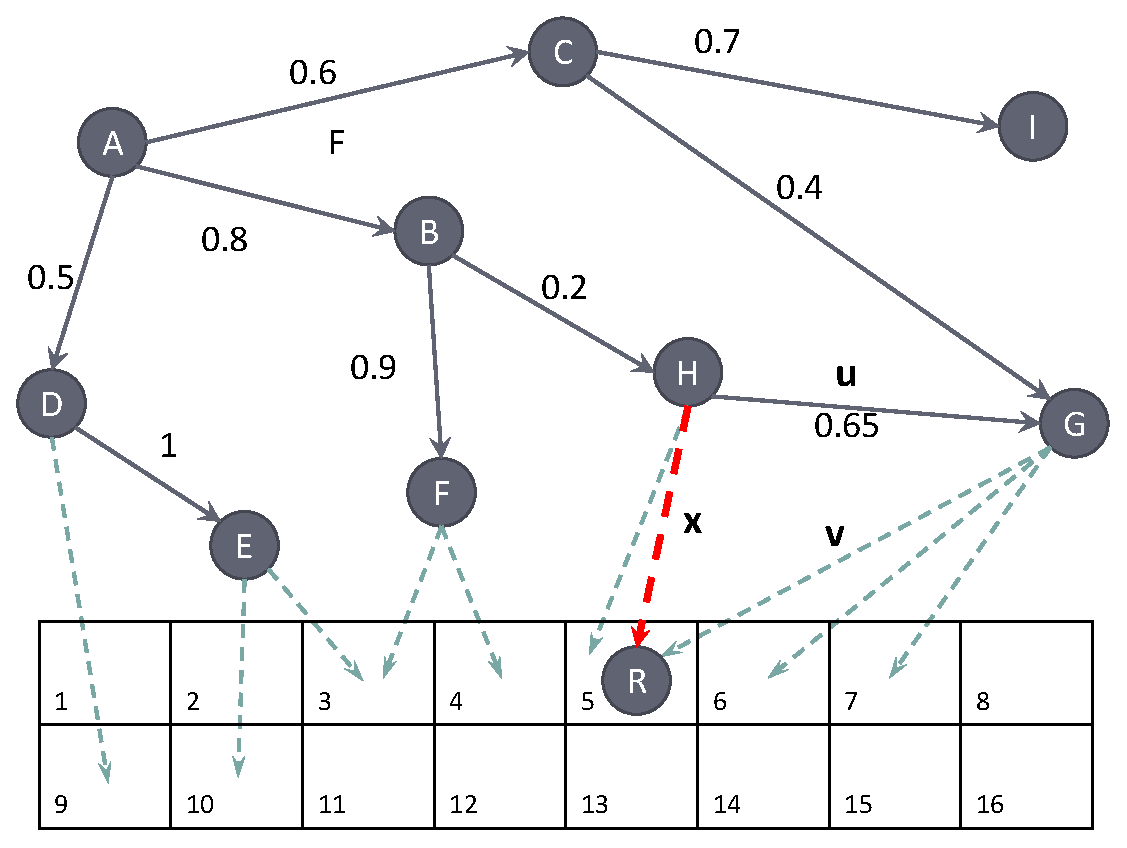
\includegraphics[width=0.88\linewidth]{images/triangle_inequality.eps}
    \caption{Triangle Inequality}
    \label{fig:tri-ine}
\end{figure}

Algorithm \ref{alg3} shows RangeReachPaths in detail. We initialize all vertices as unvisited and parent references to empty. The parent reference is used to construct the path before returning the top-k results and visited flag is used to prevent traversing the same node multiple times. The priority queue $Q$ in keyed by sum of actual distance from source and a heuristic distance to current closest vertex to a landmark. For each vertex popped from the queue, we check if it lies in R and return the result if K shortest paths are found. If not, we update keys for all existing vertices in Q with the new heuristic and we visit all unvisited neighbors of the popped vertex and see if each can reach the region R using GeoReachPaths-Spatial index. If a neighbor can reach R, and if it not already in $Q$, we compute its heuristic distance, add it to its distance from the source and insert into the $Q$. If the vertex is already in the $Q$, we simply update its key if the new distance is smaller. We proceed this way till we exhaust all vertices in the Q or find K shortest paths to R whichever is earlier. This way, we provide an iterative algorithm which doesn't traverse the entire graph to return the top-K results.

% \begin{algorithm*}[h]
% \caption{RangeReachPaths}
% \label{alg2}
% \begin{multicols}{2}
% \begin{algorithmic}[1]
% \Function{RRP}{G, s, R, K}
% 	\State $nearest\_vertices \gets []$
% 	\State \Call{INIT}{G, s}
% 	\State $Q \gets [s]$
% 	\State $best\_index \gets 0$
% 	\While{Q is not empty}
% 		\State $v \gets \Call{EXTRACT\_MIN}{Q}$
		
% 		\If{\Call{LIES\_IN}{v, R}}
% 			\State $nearest\_vertices << v$ \Comment{add v to set}
% 			\State $best\_index \gets best\_index + 1$
% 			\If{nearest\_vertices.length = K}
% 				\State \Return \Call{PATHS}{nearest\_vertices}
% 			\EndIf
% 			\For{$v \gets Q$} \Comment{Update heuristic for existing in Q}
% 				\State $v.key \gets v.d +$ HEURISTIC(u, R, best\_index)
% 			\EndFor
% 		\EndIf
		
% 		\If{v.color = WHITE}
% 			\State $v.color \gets$ BLACK
% 			\For{$u \gets G.Adj(v)$}
% 				\If{\textbf{not} \Call{LIES\_IN}{R, GRP-SPATIAL(u)}}
% 					\State \textbf{continue}
% 				\EndIf
% 				\If{u.color = WHITE}
% 					\If{u in Q}
% 						\If{u.d < v.d + WEIGHT(u, v)}
% 							\State \textbf{continue}
% 						\Else
% 							\State $u.key \gets v.d +$ WEIGHT(u, v)
% 						\EndIf
% 					\Else
% 						\State $u.parent \gets v$
% 						\State $u.d \gets v.d +$ WEIGHT(u, v)
% 						\State $u.key \gets HEURISTIC(u, R, best\_index)$
% 						\State Q.INSERT(u)
% 					\EndIf
% 				\EndIf
% 			\EndFor
% 		\EndIf
% 	\EndWhile
% \EndFunction
% \State

% \Function{HEURISTIC}{u, R, i}
% 	\State $v \gets RTREE.filter(R)$   	\Comment{vertices in R}
% 	\State \Return MAX( MIN$_i$(GRP-SOCIAL(l, u) $\forall u \in v) \forall l \in$ L)
% 	\State \Comment{$i^{th}$ minimum $u$ in $v$}
% \EndFunction
% \State

% \Function{INIT}{G, s}
% 	\State $s.key \gets 0$   	\Comment{key for priority queue}
% 	\State $s.d \gets 0$	\Comment{actual distance from source}
% 	\For{$v \gets G.V$}
% 		\State $v.color \gets$ WHITE 
% 		\State $v.parent \gets NULL$
% 	\EndFor
% \EndFunction
% \State

% \Function{LIES\_IN}{x, y}
% 	\If{x is a region}
% 		\If{x overlaps or completely falls in y}
% 			\State \Return true
% 		\EndIf
% 	\EndIf
% 	\If{x is a point \textbf{and} x falls in y}
% 		\State \Return true
% 	\EndIf
% 	\State \Return false
% \EndFunction
% \State

% \Function{PATHS}{vertices}
% 	\State $ps \gets []$ \Comment{list of paths for all vertices}
% 	\For{$u \gets vertices$}
% 		\State $p \gets []$
% 		\While{u.parent <> NULL}
% 			\State $p.prepend(u)$
% 			\State $u \gets u.parent$
% 		\EndWhile
% 		\State $p.prepend(u)$
% 		\State $ps << p$
% 	\EndFor
% \EndFunction
% \end{algorithmic}
% \end{multicols}
% \end{algorithm*}

\begin{algorithm}[t]
\caption{RangeReachPaths}
\begin{scriptsize}
\label{alg3}
\begin{algorithmic}[1]
\Function{RRP}{G, s, R, K}
	\State $nearest\_vertices \gets []$
	\State $Q \gets [s]$
	\State $best\_index \gets 0$
	\While{Q is not empty}  \label{alg:theqstart}
		\State $v \gets \Call{EXTRACT\_MIN}{Q}$
		
		\If{v lies in R}
			\State nearest\_vertices $<<$ v \Comment{add v to set}
			\State best\_index $\gets$ best\_index + 1
			\If{nearest\_vertices.length = K}
				\State \Return \Call{PATHS}{nearest\_vertices}
			\EndIf
			\For{$v \gets Q$} \Comment{Update heuristic for existing in Q}
				\State $v.key \gets v.d +$ HEURISTIC(u, R, best\_index)
			\EndFor
		\EndIf
		
		\If{v is not visited}
			\State \Call{VSIT}{G, u, v, Q}
		\EndIf
	\EndWhile	\label{alg:theqend}
\EndFunction

\Function{HEURISTIC}{u, R, i}
	\State $v \gets RTREE.filter(R)$   	\Comment{vertices in R}
	\State \Return MAX( MIN$_i$(GRP-SOCIAL(l, u) $\forall u \in v) \forall l \in$ L)
\EndFunction

% \Function{LIES\_IN}{x, y}
% 	\If{x is a region \textbf{and} x overlaps or completely falls in y}
% 		\State \Return true
% 	\EndIf
% 	\If{x is a point \textbf{and} x falls in y}
% 		\State \Return true
% 	\EndIf
% 	\State \Return false
% \EndFunction
\end{algorithmic}

\end{scriptsize}
\end{algorithm}


\begin{algorithm}[t]
\caption{Vertex Visit}
\begin{scriptsize}
\label{alg4}
\begin{algorithmic}[1]
\Function{VISIT}{G, u, v, Q}
	\For{u $\gets$ G.Adj(v)}
		\If{R does \textbf{not} lie in GRP-SPATIAL(u)}
			\State \textbf{continue}
		\EndIf
		\If{u is not visited}
			\If{u in Q}
				\If{u.d < v.d + WEIGHT(u, v)}
					\State \textbf{continue}
				\Else
					\State u.key $\gets$ v.d + WEIGHT(u, v)
				\EndIf
			\Else
				\State u.parent $\gets$ v
				\State u.d $\gets$ v.d + WEIGHT(u, v)
				\State u.key $\gets$ HEURISTIC(u, R, best\_index)
				\State Q.INSERT(u)
			\EndIf
		\EndIf
	\EndFor
\EndFunction
\end{algorithmic}

\end{scriptsize}
\end{algorithm}
